% CAGate Fig1 — Mechanism Diagram (TikZ, colorblind-safe Okabe-Ito palette)
% Generous spacing: zero overlap guaranteed
\documentclass[tikz,border=8pt]{standalone}
\usepackage{amsmath,amssymb}
\usepackage{tikz}
\usetikzlibrary{shapes.geometric, arrows.meta, positioning, backgrounds, fit, calc}

% Okabe-Ito colorblind-safe palette
\definecolor{cbBlue}{HTML}{0072B2}
\definecolor{cbOrange}{HTML}{D55E00}
\definecolor{cbGreen}{HTML}{009E73}
\definecolor{cbPurple}{HTML}{CC79A7}
\definecolor{cbDark}{HTML}{333333}
\definecolor{cbGray}{HTML}{999999}
\definecolor{cbLight}{HTML}{F5F5F5}

\begin{document}
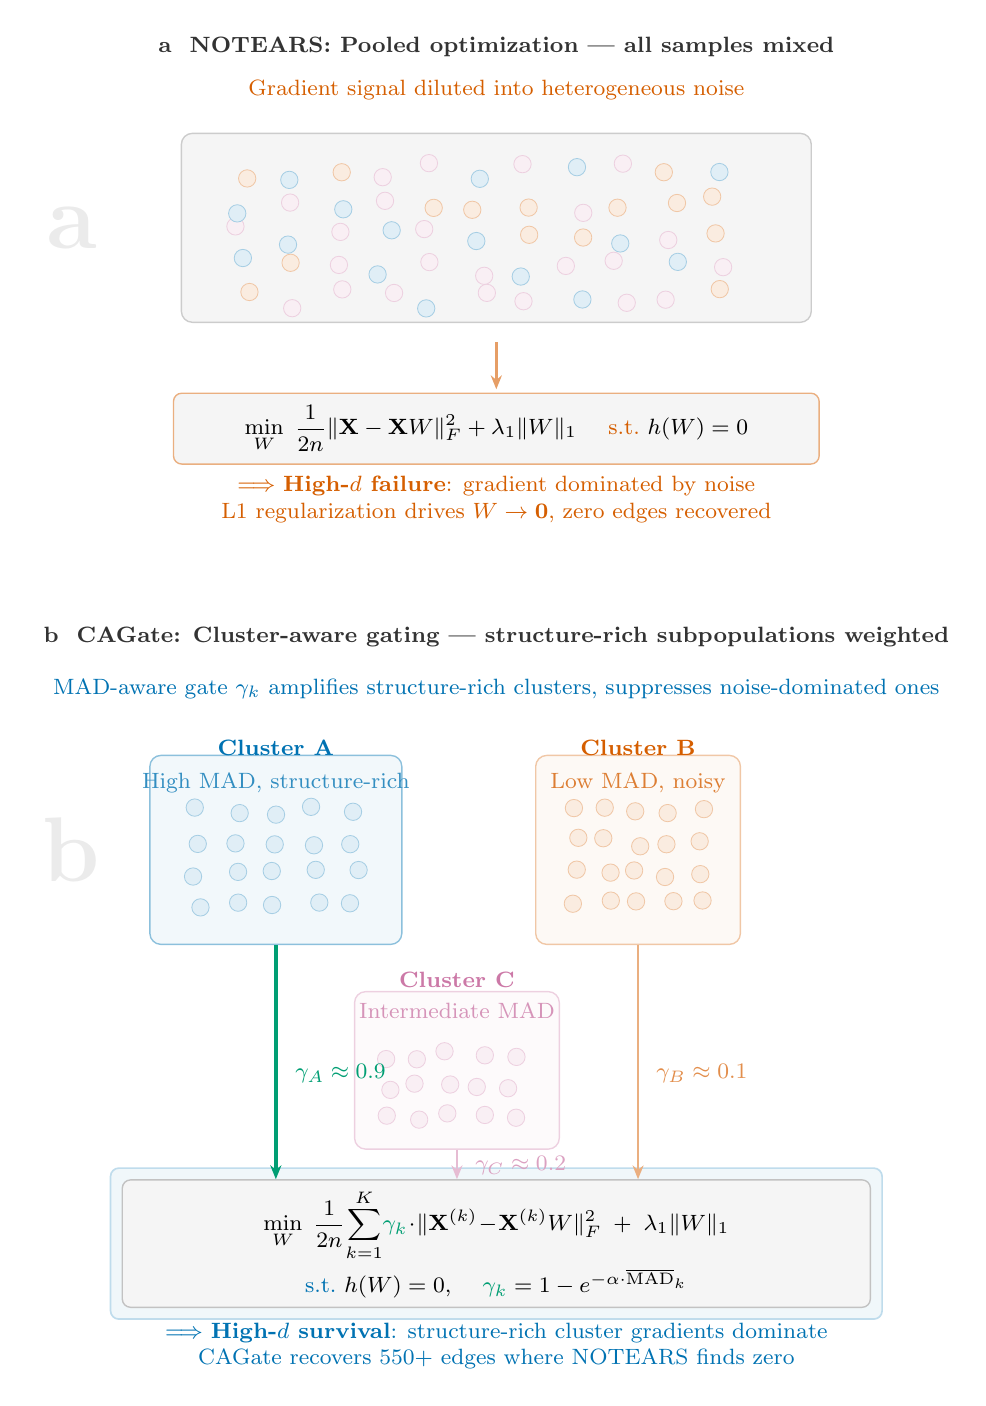
\begin{tikzpicture}[
  sample/.style={circle, draw=cbGray!50, fill=white, minimum size=0.22cm, inner sep=0pt, line width=0.3pt},
  cluster_box/.style={rectangle, draw=cbGray!50, fill=cbLight, rounded corners=4pt, minimum width=2.6cm, minimum height=2.0cm, line width=0.5pt},
  arrow/.style={-{Stealth[length=5pt,width=4pt]}, line width=1.0pt},
  loss_box/.style={rectangle, draw=cbGray!60, fill=cbLight, rounded corners=3pt, minimum width=9.2cm, minimum height=0.9cm, align=center, font=\footnotesize, line width=0.5pt},
  note/.style={font=\footnotesize, text=cbDark},
  title/.style={font=\bfseries\footnotesize, text=cbDark},
  cluster_label/.style={font=\footnotesize\bfseries},
  % Use picture bounding box to prevent clips
]

% ══════════════════════════════════════════
% PANEL (a): NOTEARS — Pooled Optimization
% ══════════════════════════════════════════
\node[title] at (0, 0) {\textbf{a}~~NOTEARS: Pooled optimization — all samples mixed};
\node[note, text=cbOrange] at (0, -0.55) {Gradient signal diluted into heterogeneous noise};

% Large pooled cluster box
\node[cluster_box, minimum width=8.0cm, minimum height=2.4cm] (pool) at (0, -2.3) {};

% Sample dots inside the pooled box (randomized colors for heterogeneity)
\foreach \x in {-3.2,-2.6,-2.0,-1.4,-0.8,-0.2,0.4,1.0,1.6,2.2,2.8} {
  \foreach \y in {-3.2,-2.8,-2.4,-2.0,-1.6} {
    \pgfmathsetmacro\dx{rnd*0.25-0.125}
    \pgfmathsetmacro\dy{rnd*0.25-0.125}
    \pgfmathparse{int(rnd*3)}
    \ifcase\pgfmathresult
      \node[sample, fill=cbOrange!12, draw=cbOrange!35] at (\x+\dx, \y+\dy) {};
    \or
      \node[sample, fill=cbBlue!12, draw=cbBlue!35] at (\x+\dx, \y+\dy) {};
    \or
      \node[sample, fill=cbPurple!12, draw=cbPurple!35] at (\x+\dx, \y+\dy) {};
    \fi
  }
}

% Arrow pool -> loss
\draw[arrow, cbOrange!60] (0, -3.75) -- (0, -4.35);

% NOTEARS loss formula
\node[loss_box, draw=cbOrange!50, minimum width=8.2cm] (loss_a) at (0, -4.85) {
  $\displaystyle \min_W \; \frac{1}{2n}\|\mathbf{X} - \mathbf{X}W\|_F^2 + \lambda_1\|W\|_1$
  \quad {\footnotesize\textcolor{cbOrange}{s.t.}~$h(W)=0$}};

% Failure callout
\node[note, text=cbOrange, align=center] at (0, -5.75) {
  $\Longrightarrow$\ \textbf{High-$d$ failure}: gradient dominated by noise\\
  L1 regularization drives $W \to \mathbf{0}$, zero edges recovered};

% ══════════════════════════════════════════
% PANEL (b): CAGate — Cluster-Aware Gating
% ══════════════════════════════════════════
\node[title] at (0, -7.5) {\textbf{b}~~CAGate: Cluster-aware gating — structure-rich subpopulations weighted};
\node[note, text=cbBlue] at (0, -8.15) {MAD-aware gate $\gamma_k$ amplifies structure-rich clusters, suppresses noise-dominated ones};

% ── Top row: Cluster A (structure-rich) and Cluster B (noisy) ──
% Cluster A — high MAD, high weight
\node[cluster_box, fill=cbBlue!5, draw=cbBlue!45, minimum width=3.2cm, minimum height=2.4cm] (clA) at (-2.8, -10.2) {};
\node[cluster_label, text=cbBlue] at (-2.8, -8.9) {Cluster A};
\node[note, text=cbBlue!80] at (-2.8, -9.35) {High MAD, structure-rich};
% Samples inside Cluster A
\foreach \x in {-3.8,-3.3,-2.8,-2.3,-1.8} {
  \foreach \y in {-10.9,-10.5,-10.1,-9.7} {
    \pgfmathsetmacro\dx{rnd*0.12-0.06}
    \pgfmathsetmacro\dy{rnd*0.12-0.06}
    \node[sample, fill=cbBlue!12, draw=cbBlue!35] at (\x+\dx, \y+\dy) {};
  }
}

% Cluster B — low MAD, suppressed
\node[cluster_box, fill=cbOrange!4, draw=cbOrange!35, minimum width=2.6cm, minimum height=2.4cm] (clB) at (1.8, -10.2) {};
\node[cluster_label, text=cbOrange] at (1.8, -8.9) {Cluster B};
\node[note, text=cbOrange!80] at (1.8, -9.35) {Low MAD, noisy};
\foreach \x in {1.0,1.4,1.8,2.2,2.6} {
  \foreach \y in {-10.9,-10.5,-10.1,-9.7} {
    \pgfmathsetmacro\dx{rnd*0.12-0.06}
    \pgfmathsetmacro\dy{rnd*0.12-0.06}
    \node[sample, fill=cbOrange!12, draw=cbOrange!35] at (\x+\dx, \y+\dy) {};
  }
}

% ── Bottom row: Cluster C (intermediate) ──
\node[cluster_box, fill=cbPurple!4, draw=cbPurple!35, minimum width=2.6cm, minimum height=2.0cm] (clC) at (-0.5, -13.0) {};
\node[cluster_label, text=cbPurple] at (-0.5, -11.85) {Cluster C};
\node[note, text=cbPurple!80] at (-0.5, -12.25) {Intermediate MAD};

\foreach \x in {-1.4,-1.0,-0.6,-0.2,0.2} {
  \foreach \y in {-13.6,-13.2,-12.8} {
    \pgfmathsetmacro\dx{rnd*0.12-0.06}
    \pgfmathsetmacro\dy{rnd*0.12-0.06}
    \node[sample, fill=cbPurple!12, draw=cbPurple!35] at (\x+\dx, \y+\dy) {};
  }
}

% ── CAGate loss box ──
\node[loss_box, minimum width=9.5cm] (loss_b) at (0, -15.2) {%
  $\displaystyle \min_W \; \frac{1}{2n}\!\sum_{k=1}^{K}\! \textcolor{cbGreen}{\gamma_k}\!\cdot\!\|\mathbf{X}^{(k)}\!-\!\mathbf{X}^{(k)}W\|_F^2 \;+\; \lambda_1\|W\|_1$
  \\[2pt]
  {\footnotesize\textcolor{cbBlue}{s.t.}~$h(W)=0$,
   \quad $\textcolor{cbGreen}{\gamma_k}=1-e^{-\alpha\cdot\overline{\mathrm{MAD}}_k}$}};

% ── Gate arrows from clusters to loss box ──
\draw[arrow, cbGreen, line width=1.5pt] (clA.south) -- (clA.south |- loss_b.north)
  node[pos=0.55, right=3pt, font=\footnotesize\bfseries, text=cbGreen] {$\gamma_A\approx 0.9$};
\draw[arrow, cbOrange!50, line width=0.5pt] (clB.south) -- (clB.south |- loss_b.north)
  node[pos=0.55, right=3pt, font=\footnotesize, text=cbOrange!70] {$\gamma_B\approx 0.1$};
\draw[arrow, cbPurple!50, line width=0.6pt] (clC.south) -- (clC.south |- loss_b.north)
  node[pos=0.55, right=3pt, font=\footnotesize, text=cbPurple!70] {$\gamma_C\approx 0.2$};

% Highlight ring around loss formula
\begin{scope}[on background layer]
\node[rectangle, rounded corners=3pt, fill=cbBlue!6, draw=cbBlue!25, line width=0.6pt,
      inner sep=4pt, fit=(loss_b)] {};
\end{scope}

% ── Result callout ──
\node[note, text=cbBlue, align=center] at (0, -16.5) {
  $\Longrightarrow$\ \textbf{High-$d$ survival}: structure-rich cluster gradients dominate\\
  CAGate recovers 550+ edges where NOTEARS finds zero};

% ── Panel watermarks ──
\node[font=\huge\bfseries, text=cbGray!20, scale=1.6] at (-5.4, -2.3) {a};
\node[font=\huge\bfseries, text=cbGray!20, scale=1.6] at (-5.4, -10.2) {b};

\end{tikzpicture}
\end{document}
